<latex packages="{tikz}" ><![CDATA[
\centerline{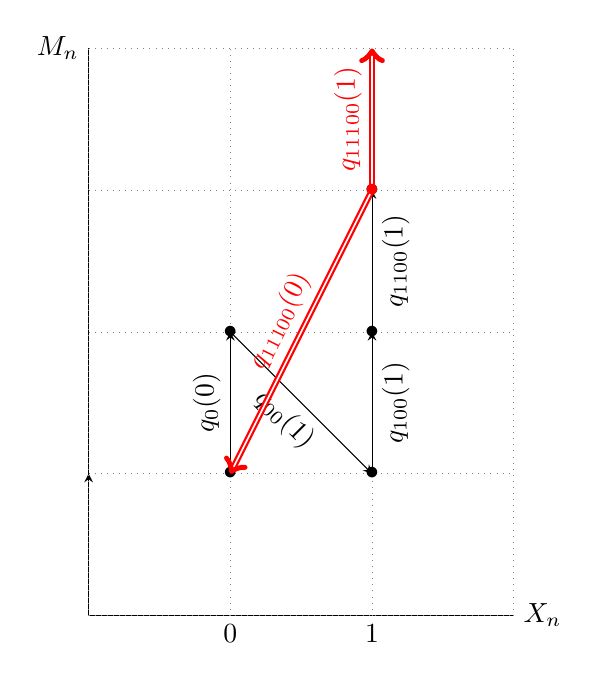
\begin{tikzpicture}[scale=1.8]
\draw (0,0) -- (0,4) ;
\draw [>=stealth,->] (0,0) -- (0,1) ;
\draw (0,0) -- (3,0) ;
\draw [dotted, very thin, gray] (0,0) grid (3,4);
\draw (3,0) node[right]{$X_n$} ;
\draw (0,4) node[left]{$M_n$} ;
\draw (1,0) node[below]{0};
\draw (2,0) node[below]{1};\draw (1, 1) node {$\bullet$};
\draw [>=stealth, ->] (1, 1) -- (1, 2) node[midway,above,sloped]{$q_{0}(0)$};
\draw (1, 2) node {$\bullet$};
\draw [>=stealth, ->] (1, 2) -- (2, 1) node[midway,below,sloped]{$q_{00}(1)$};
\draw (2, 1) node {$\bullet$};
\draw [>=stealth, ->] (2, 1) -- (2, 2) node[midway,below,sloped]{$q_{100}(1)$};
\draw (2, 2) node {$\bullet$};
\draw [>=stealth, ->] (2, 2) -- (2, 3) node[midway,below,sloped]{$q_{1100}(1)$};
\draw (2, 3) node {$\bullet$};
\draw [draw=red, fill=red, ->, double,thick] (2, 3) -- (1, 1) node[midway,above,sloped]{{\color{red}$q_{11100}(0)$}};
\draw [draw=red, fill=red, ->, double,thick] (2, 3) -- (2, 4) node[midway,above,sloped]{{\color{red}$q_{11100}(1)$}};
\draw (2, 3) node {{\color{red}$\bullet$}};
\end{tikzpicture}}
\centerline{...100111}]]>
</latex>